\part{13/1}

\section{Wiederholung}
\begin{itemize}
  \item relative Häufigkeit: Aussage über ein schon durchgeführtes Zufallsexperiment
  \item Wahrscheinlichkeit: Aussage über zukünftige Zufallsversuche
\end{itemize}
\begin{exercise}{456/5}
  \begin{gather*}
    F = \{(1, 1), (2, 1), (3, 1), (4, 1)\}
  \end{gather*}
  \item [a]
  \begin{gather*}
    E = \{(1, 1), (1, 2), (2, 1)\} \\\\
    F \colon \text{Die zweite Kugel trägt eine $1$} \\
    E \Leftrightarrow \text{Die Summe der Zahlen ist größer als $3$} \\\\
    P(E) = (\frac{2}{6} \cdot \frac{2}{6}) + (\frac{2}{6} \cdot \frac{1}{6}) + (\frac{1}{6} \cdot \frac{2}{6}) = \frac{2}{9} = 0.\overline{2} \\
    P(F) = (\frac{2}{6} \cdot \frac{2}{6}) + (\frac{1}{6} \cdot \frac{2}{6}) + (\frac{2}{6} \cdot \frac{2}{6}) + (\frac{1}{6} \cdot \frac{2}{6}) = P(1) = \frac{2}{6} = \frac{1}{3} = 0.\overline{3}
  \end{gather*}
  \item [b]
  \begin{gather*}
    E \cap F = \{(1, 1), (2, 1)\} \\
    P(E \cap F) = (\frac{2}{6} \cdot \frac{2}{6}) + (\frac{1}{6} \cdot \frac{2}{6}) = \frac{1}{6} = 0.1\overline{6}
  \end{gather*}
  \item [c]
  \begin{gather*}
    E \cup F = \{(1, 1), (1, 2), (2, 1), (3, 1), (4, 1)\} \\
    P(E \cup F) = (\frac{2}{6} \cdot \frac{2}{6}) + (\frac{2}{6} \cdot \frac{1}{6}) + (\frac{1}{6} \cdot \frac{2}{6}) + (\frac{2}{6} \cdot \frac{2}{6}) + (\frac{1}{6} \cdot \frac{2}{6}) = \frac{7}{18} = 0.3\overline{8}
  \end{gather*}
\end{exercise}
\begin{exercise}{456/7}
  \item [a]
  \begin{gather*}
    \text{Gegenwahrscheinlichkeit (keine Sechs werfen): } P(\neg E) = (\frac{5}{6})^5 \approx 0.40 \\
    P(E) = 1 - P(\neg E) = 1 - (\frac{5}{6})^5 \approx 0.60
  \end{gather*}
  \item [b]
  \begin{gather*}
    P = \frac{6}{6} \cdot \frac{5}{6} \cdot \frac{4}{6} \cdot \frac{3}{6} \cdot \frac{2}{6} = \approx 0.09
  \end{gather*}
  \item [c]
  \begin{gather*}
    P = (\frac{5}{6})^4 \cdot \frac{1}{6} \approx 0.08
  \end{gather*}
\end{exercise}
\begin{exercise}{456/9}
  \item [a]
  \begin{gather*}
    P = \frac{1}{13983816} \approx 7.15 \cdot 10^{-8}
  \end{gather*} \\\\
  Bemerkung: Ein Zufallsversuch heißt Laplace-Versuch, wenn alle Ergebnisse gleich wahrscheinlich sind.
  \begin{gather*}
    S = \{e_1, e_2, ..., e_n\} \qquad |S| = n \qquad P(e_i) = \frac{1}{n} \\
    E = \{e_1, ...\} \qquad |E| = k \qquad P(E) = \frac{k}{n}
  \end{gather*}
  $\Rightarrow$ Gleichverteilung
  \item [b]
  \begin{gather*}
    E = \{(1,2,3,4,5,6), (2,3,4,5,6,7), ..., (44,45,46,47,48,49)\} \\
    |E| = 44 \\
    P(E) = \frac{|E|}{|S|} = \frac{44}{13983816} \approx 3.15 \cdot 10^{-6}
  \end{gather*}
  \item [c]
  \begin{gather*}
    P = \frac{43}{49} \cdot \frac{42}{48} \cdot \frac{41}{47} \cdot \frac{40}{46} \cdot \frac{39}{45} \cdot \frac{38}{44} \approx 0.436
  \end{gather*}
\end{exercise}
\begin{exercise}{456/10}
  \item [a]
  \begin{gather*}
    \text{Anteil nach $10$ Tagen: } 0.85^{10} \approx 0.197 \\
    0.85^t = 0.5 \quad\Rightarrow\quad t = log_{0.85}(0.5) \approx 4.265
  \end{gather*}
  \item [b]
  \begin{gather*}
    (1 - p)^8 = 0.5 \quad\Rightarrow\quad p = 1 - \sqrt[8]{(0.5)} \approx 0.083
  \end{gather*}
\end{exercise}
\section{Abzählverfahren}
Bis auf Weiteres gilt: Die Zufallsversuche sind Laplace-Versuche. \\
Anzahl der Ergebnisse $N \quad\Rightarrow\quad P = \frac{1}{N} \quad\text{(Ergebniswahrscheinlichkeit)}$ \\\\
Ziehe $k$ mal aus einer Urne mit $n$ unterscheidbaren Kugeln:
\begin{itemize}
  \item mit Zurücklegen, unter Beachtung der Reihenfolge
  \begin{gather*}
    N = n^k
  \end{gather*}
  \item ohne Zurücklegen, unter Beachtung der Reihenfolge
  \begin{gather*}
    N = n \cdot (n - 1) \cdot (n - 2) \cdot ... \cdot \underbrace{(n - k + 1)}_{\mathclap{\text{übrige Kugeln vor dem $k$-ten Zug}}} = \frac{n!}{(n - k)!}
  \end{gather*}
  \item ohne Zurücklegen, ohne Beachtung der Reihenfolge \\\\
  Es werden jeweils $k!$ (Permutationen) Ergebnisse zu einem Ereignis zusammengefasst:
  \begin{gather*}
    N = \frac{n!}{(n - k)! \cdot k!} = \begin{pmatrix}n \\ k\end{pmatrix} \text{ (Binomialkoeffizient)}
  \end{gather*} \\
  Die Wahrscheinlichkeit für einen 6er im Lotto:
  \begin{gather*}
    p = \frac{1}{\begin{pmatrix}49 \\ 6\end{pmatrix}} \approx \frac{1}{14000000}
  \end{gather*}
  Die Wahrscheinlichkeit für einen 4er im Lotto (``Lottoproblem''):
  \begin{gather*}
    p = \frac{\begin{pmatrix}6 \\ 4\end{pmatrix} \cdot \begin{pmatrix}43 \\ 2\end{pmatrix}}{\begin{pmatrix}49 \\ 6\end{pmatrix}} = \frac{13545}{\begin{pmatrix}49 \\ 6\end{pmatrix}} \approx \frac{1}{1000}
  \end{gather*}
  \qquad (Wähle $4$ aus den $6$ Richtigen und $2$ aus den $43$ Falschen)
\end{itemize}
\begin{exercise}{460/1}
  \item [a]
  \begin{gather*}
    n = 2 \quad k = 6 \quad N = 2^6 = 64
  \end{gather*}
  \item [b]
  \begin{gather*}
    n = 4 \quad k = 4 \quad N = \frac{4!}{(4 - 4)!} = 4! = 24
  \end{gather*}
  \item [c]
  \begin{gather*}
    n = 3 \quad k = 5 \quad N = 3^5 = 243
  \end{gather*}
  \item [d]
  \begin{gather*}
    n = 10 \quad k = 2 \quad N = \begin{pmatrix}10 \\ 2\end{pmatrix} = 45
  \end{gather*}
\end{exercise}
\begin{exercise}{460/2}
  \item [a]
  \begin{gather*}
    n = 4 \quad k = 4 \quad N = 4^4 = 256
  \end{gather*}
  \item [b]
  \begin{gather*}
    p_1 = \frac{1}{2} \cdot \frac{1}{4} \cdot \frac{1}{8} \cdot \frac{1}{8} = \frac{1}{512} \\
    p_2 = \frac{4!}{p_1} = \frac{3}{64} \\
    p_3 = 1 - (\frac{1}{2})^4 = \frac{15}{16}
  \end{gather*}
\end{exercise}
\begin{exercise}{460/3}
  \item [a] Die Reihenfolge der Ziffern entspricht der Reihenfolge der Spiele.
  \item [b]
  \begin{gather*}
    p = (\frac{1}{3})^{11} = \frac{1}{177147} \approx 5.65 \cdot 10^{-6}
  \end{gather*}
  Annahme: Heimsieg, Gastsieg und Unentschieden sind jeweils gleich wahrscheinlich.
  \item [c]
  \begin{gather*}
    N = (\frac{2}{3})^{11} \cdot 3^{11} = 2^{11} = 2048
  \end{gather*}
\end{exercise}
\begin{exercise}{460/5}
  \begin{gather*}
    N = \frac{12!}{(12 - 3)!} = 1320
  \end{gather*}
\end{exercise}
\begin{exercise}{461/8}
  \item [a]
  \begin{gather*}
    N = 5! = 120
  \end{gather*}
  \item [b]
  \begin{gather*}
    p = \frac{1}{5}
  \end{gather*}
  \item [c]
  \begin{gather*}
    \frac{1}{5} \cdot \frac{1}{4} = \frac{1}{20}
  \end{gather*}
\end{exercise}
\begin{exercise}{461/11}
  \item [a]
  \begin{gather*}
    p = \frac{6}{49} \cdot \frac{5}{48} \cdot \frac{4}{47} \cdot \frac{3}{46} \cdot \frac{43}{45} \cdot \frac{42}{44} \approx 6.46 \cdot 10^{-5}
  \end{gather*}
  \item [b]
  \begin{gather*}
    rrrrff, rrrfrf, rrfrrf, rfrrrf, frrrrf, \\
    rrrffr, rrfrfr, rfrrfr, frrrfr, \\
    rrffrr, rfrfrr, frrfrr, \\
    rffrrr, frfrrr, \\
    ffrrrr
  \end{gather*}
  \item [c]
  \begin{gather*}
    p_4 \approx 15 \cdot 6.46 \cdot 10^{-5} \approx 9.69 \cdot 10^{-4}
  \end{gather*}
  \item [d]
  \begin{gather*}
    p_2 = \begin{pmatrix}6 \\ 2\end{pmatrix} \cdot (\frac{6}{49} \cdot \frac{5}{48} \cdot \frac{43}{47} \cdot \frac{42}{46} \cdot \frac{41}{45} \cdot \frac{40}{44}) \approx 0.13
  \end{gather*}
  \item [e]
  \begin{gather*}
    p_0 = \begin{pmatrix}6 \\ 0\end{pmatrix} \cdot (\frac{43}{49} \cdot \frac{42}{48} \cdot \frac{41}{47} \cdot \frac{40}{46} \cdot \frac{39}{45} \cdot \frac{38}{44}) \approx 0.44 \\
    p_1 = \begin{pmatrix}6 \\ 1\end{pmatrix} \cdot (\frac{6}{49} \cdot \frac{43}{48} \cdot \frac{42}{47} \cdot \frac{41}{46} \cdot \frac{40}{45} \cdot \frac{39}{44}) \approx 0.41 \\
    p_{\geq 3} = 1 - (p_0 + p_1 + p_2) \approx 1.86 \cdot 10^{-2} \\\\
    p_{50Sp.} = 1 - (p_0 + p_1 + p_2)^{50} \approx 0.61 \\
    p_{100Sp.} = 1 - (p_0 + p_1 + p_2)^{100} \approx 0.85 \\
    p_{1000Sp.} = 1 - (p_0 + p_1 + p_2)^{1000} \approx 1.00
  \end{gather*}
\end{exercise}
\begin{exercise}{461/10}
  \item [a]
  \begin{gather*}
    p = \begin{pmatrix}6 \\ 6\end{pmatrix} \cdot (\frac{6}{45} \cdot \frac{5}{44} \cdot \frac{4}{43} \cdot \frac{3}{42} \cdot \frac{2}{41} \cdot \frac{1}{40}) = \frac{1}{\begin{pmatrix}45 \\ 6\end{pmatrix}} \approx 1.23 \cdot 10^{-7}
  \end{gather*}
  \item [b]
  \begin{gather*}
    N = \begin{pmatrix}5 \\ 2\end{pmatrix} = 10
  \end{gather*}
  \item [c]
  \begin{gather*}
    N = \begin{pmatrix}1000 \\ 2\end{pmatrix} = 4.995 \cdot 10^{5}
  \end{gather*}
\end{exercise}
\subsubsection{AB Grundbegriffe der Wahrscheinlichkeitsrechnung}
\begin{exercise}{AB/12}
  \begin{gather*}
    p = \frac{6}{7} \cdot \frac{4}{5} \cdot \frac{2}{3} \approx 0.46
  \end{gather*}
\end{exercise}
\begin{exercise}{AB/17}
  \item [a]
  \begin{gather*}
    N = \begin{pmatrix}16 \\ 3\end{pmatrix} \cdot \begin{pmatrix}8 \\ 2\end{pmatrix} = 39200
  \end{gather*}
  \item [b]
  \begin{gather*}
    N = \begin{pmatrix}24 \\ 5\end{pmatrix} - \begin{pmatrix}16 \\ 5\end{pmatrix} = 38136
  \end{gather*}
\end{exercise}
\begin{exercise}{AB/20}
  \begin{gather*}
    p_{3r} = \frac{\begin{pmatrix}5 \\ 3\end{pmatrix} \cdot \begin{pmatrix}15 \\ 5\end{pmatrix}}{\begin{pmatrix}20 \\ 8\end{pmatrix}} \approx 0.2384 \\
    p_{\geq 4r} = \frac{\begin{pmatrix}5 \\ 4\end{pmatrix} \cdot \begin{pmatrix}15 \\ 4\end{pmatrix}}{\begin{pmatrix}20 \\ 8\end{pmatrix}} + \frac{\begin{pmatrix}5 \\ 5\end{pmatrix} \cdot \begin{pmatrix}15 \\ 3\end{pmatrix}}{\begin{pmatrix}20 \\ 8\end{pmatrix}} \approx 0.0578
  \end{gather*}
\end{exercise}
\begin{exercise}{AB/21}
  \begin{gather*}
    p_2 = \frac{\begin{pmatrix}10 \\ 2\end{pmatrix} \cdot \begin{pmatrix}90 \\ 3\end{pmatrix}}{\begin{pmatrix}100 \\ 5\end{pmatrix}} \approx 0.0702 \\\\
    p_{\geq 3} = p_3 + p_4 + p_5 \\
    \;= \frac{\begin{pmatrix}10 \\ 3\end{pmatrix} \cdot \begin{pmatrix}90 \\ 2\end{pmatrix} + \begin{pmatrix}10 \\ 4\end{pmatrix} \cdot \begin{pmatrix}90 \\ 1\end{pmatrix} + \begin{pmatrix}10 \\ 5\end{pmatrix} \cdot \begin{pmatrix}90 \\ 0\end{pmatrix}}{\begin{pmatrix}100 \\ 5\end{pmatrix}} \approx 0.0066
  \end{gather*}
\end{exercise}
\begin{exercise}{AB/11}
  \item [a]
  \begin{gather*}
    N = (4 + 5 + 3)! = 479001600
  \end{gather*}
  \item [b]
  \begin{gather*}
    N = 3! \cdot 4! \cdot 5! \cdot 3! = 103680
  \end{gather*}
\end{exercise}
\begin{exercise}{AB/13}
  \begin{gather*}
    t = \frac{26!}{10^6} \approx 4.0329 \cdot 10^{20}ms \approx 1.2780 \cdot 10^{10}y \approx 0.93 \cdot \text{Alter des Universums}
  \end{gather*}
\end{exercise}
\begin{exercise}{AB/23}
  \begin{gather*}
    p_3 = \frac{\begin{pmatrix}4 \\ 3\end{pmatrix} \cdot \begin{pmatrix}12 \\ 1\end{pmatrix}}{\begin{pmatrix}16 \\ 4\end{pmatrix}} \approx 2.6374 \cdot 10^{-2} \\
    p_4 = \frac{\begin{pmatrix}4 \\ 4\end{pmatrix} \cdot \begin{pmatrix}12 \\ 0\end{pmatrix}}{\begin{pmatrix}16 \\ 4\end{pmatrix}} \approx 5.4945 \cdot 10^{-4} \\
    Erw = 1 - (10 \cdot p_3 + 1000 \cdot p_4) \approx 0.19
  \end{gather*}
\end{exercise}
\section{Bedingte Wahrscheinlichkeit}
Aus einer Urne mit $6$ roten und $4$ blauen Kugeln werden $2$ Kugeln ohne Zurücklegen gezogen.
\begin{gather*}
  \begin{tikzpicture}[grow=down]
    \tikzstyle{level 1} = [level distance=2.5cm, sibling distance=6cm]
    \tikzstyle{level 2} = [level distance=2.5cm, sibling distance=3cm]
    \tikzstyle{level 3} = [level distance=2.5cm, sibling distance=1.5cm]
    \node {1. Zug}
      child {
        node {2. Zug}
        child {
          node {$({\color{blue}b}, {\color{blue}b})$}
          edge from parent
          node[above left] {\color{blue}$\frac{3}{9}$}
        }
        child {
          node {$({\color{blue}b}, {\color{red}r})$}
          edge from parent
          node[above right] {\color{red}$\frac{6}{9}$}
        }
        edge from parent
        node[above left] {\color{blue}$\frac{4}{10}$}
      }
      child {
        node {2. Zug}
        child {
          node {$({\color{red}r}, {\color{blue}b})$}
          edge from parent
          node[above left] {\color{blue}$\frac{4}{9}$}
        }
        child {
          node {$({\color{red}r}, {\color{red}r})$}
          edge from parent
          node[above right] {\color{red}$\frac{5}{9}$}
        }
        edge from parent
        node[above right] {\color{red}$\frac{6}{10}$}
      };
    \end{tikzpicture}
\end{gather*}
\begin{gather*}
  E \colon \text{rot im ersten Zug} \qquad P(E) = \frac{6}{10} \\
  F \colon \text{rot im zweiten Zug} \qquad P(F) = \frac{4}{10} \cdot \frac{6}{9} + \frac{6}{10} \cdot \frac{5}{9} = \frac{3}{5} \\\\
  P_E(F) = \frac{5}{9} \qquad \text{Wahrscheinlichkeit für Ereignis $F$, unter der Voraussetzung,} \\
  \qquad\qquad\qquad\quad\text{dass Ereignis $E$ zurvor eingetreten ist}
\end{gather*}
\subsection{Statistische Unabhängigkeit}
Wenn gilt, dass $P_E(F) = P(F)$, dann sagt man die Ereignisse $E$ und $F$ sind statistisch unabhängig.
\begin{gather*}
  E \colon \text{rot im ersten Zug} \qquad P(E) = \frac{6}{10} \\
  F \colon \text{rot im zweiten Zug} \qquad P(F) = \frac{3}{5} \\\\
  P_E(F) = \frac{5}{9} \neq P(F) = \frac{3}{5}
\end{gather*}
Die Wahrscheinlichkeit, dass rot im zweiten Zug gezogen wird unter der Bedingung, dass rot schon im ersten Zug gezogen wurde, ist ungleich der Wahrscheinlichkeit, dass allgemein rot im zweiten Zug gezogen wird. \\
$E$ und $F$ sind statistisch abhängig. \\
\begin{gather*}
  \overline{E} \colon \text{blau im ersten Zug} \\
  \overline{F} \colon \text{blau im zweiten Zug} \\\\
  P_{\overline{E}}(F) = \frac{6}{9} \neq P(F) = \frac{3}{5} \\
  P_E(\overline{F}) = \frac{4}{9} \neq P(\overline{F}) = \frac{2}{5} \\
  P_{\overline{E}}(\overline{F}) = \frac{3}{9} \neq P(\overline{F}) = \frac{2}{5}
\end{gather*}
\begin{exercise}{475/1}
  \item [a]
  \begin{gather*}
    P = 0.98^4 \approx 0.9224
  \end{gather*}
  \item [b]
  Wenn bei einem Fahrzeug eine Panne auftritt, besteht die Möglichkeit, dass dies auf ein besonders anfälliges Fahrzeugteil oder einen Produktionsfehler zurückzuführen ist, welches/r sich auch in den anderen drei Fahrzeugen befindet.
\end{exercise}
\newpage
\begin{exercise}{475/2}
  \item [a]
  \begin{gather*}
    P(E) = \frac{3}{5} \qquad P(F) = \frac{2}{5} \\
    E \cap F = \{(a_1, h_1), (a_1, h_2), (a_2, h_1), ..., (a_3, h_2)\} \qquad |E \cap F| = 6 \\
    P(E \cap F) = \frac{|E \cap F|}{5^2} = P(E) \cdot P(F) = \frac{6}{25}
  \end{gather*}
  \item [b]
  \begin{gather*}
    P(E) = \frac{3}{5} \qquad P(F) = \frac{3}{5} \cdot \frac{2}{4} + \frac{2}{5} \cdot \frac{1}{4} = 0.34 \\
    P(E \cap F) = \frac{3}{5} \cdot \frac{2}{4} = 0.3 \neq P(E) \cdot P(F) = 0.204 \\
    P_E(F) = \frac{2}{4} = \frac{1}{2}
  \end{gather*}
\end{exercise}
\subsubsection{Vierfelder-Tafel}
\begin{gather*}
  E \colon \text{Raucher} \qquad \overline{E} \colon \text{Nichtraucher} \\
  F \colon \text{mit Gewicht zufrieden} \qquad \overline{F} \colon \text{mit Gewicht unzufrieden}
\end{gather*}
\begin{tabular}{c|c|c|c}
  & $F$ & $\overline{F}$ & \\ \hline
  $E$ & $P(E \cap F)$ & $P(E \cap \overline{F})$ & $P(E)$ \\ \hline
  $\overline{E}$ & $P(\overline{E} \cap F)$ & $P(\overline{E} \cap \overline{F})$ & $P(\overline{E})$ \\ \hline
  & $P(F)$ & $P(\overline{F})$ & $100\%$
\end{tabular}
\begin{gather*}
  P_E(F) = \frac{P(E \cap F)}{P(E)}
\end{gather*}
\begin{exercise}{476/11}
  \begin{gather*}
    P(\text{V. h.} \cap \text{S. h.}) = \frac{471}{1000} = 47.1\% \\
    P(\text{V. h}) \cdot P(\text{S. h.}) = \frac{622}{1000} \cdot \frac{619}{1000} \approx 38.5\% \\\\
    P(\text{V. h.} \cap \text{S. h.}) \neq P(\text{V. h}) \cdot P(\text{S. h.}) \quad\Rightarrow\quad \text{statistisch abhängig}
  \end{gather*}
\end{exercise}
\subsection{Der Satz von Bayes}
\begin{gather*}
  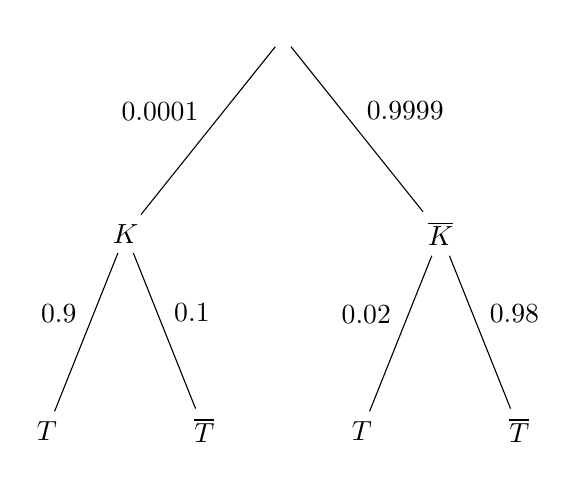
\begin{tikzpicture}[grow=down]
    \tikzstyle{level 1} = [level distance=2.5cm, sibling distance=4cm]
    \tikzstyle{level 2} = [level distance=2.5cm, sibling distance=2cm]
    \tikzstyle{level 3} = [level distance=2.5cm, sibling distance=1cm]
    \node {}
      child {
        node {$K$}
        child {
          node {$T$}
          edge from parent
          node[above left] {$0.9$}
        }
        child {
          node {$\overline{T}$}
          edge from parent
          node[above right] {$0.1$}
        }
        edge from parent
        node[above left] {$0.0001$}
      }
      child {
        node {$\overline{K}$}
        child {
          node {$T$}
          edge from parent
          node[above left] {$0.02$}
        }
        child {
          node {$\overline{T}$}
          edge from parent
          node[above right] {$0.98$}
        }
        edge from parent
        node[above right] {$0.9999$}
      };
    \end{tikzpicture}
\end{gather*}
\begin{gather*}
  P_K(T) = 0.90 \colon \text{Sensitivität des Tests} \\
  P_{\overline{K}}(\overline{T}) = 0.98 \colon \text{Spezifität des Tests} \\\\
  K \colon \text{krank} \qquad T \colon \text{positiver Test} \\
  P_T(K) \colon \text{Wahrscheinlichkeit, krank zu sein, wenn der Test positiv ausfällt} \\\\
  P_T(K) = \frac{P(K \cap T)}{P(T)} = \frac{P(K) \cdot P_K(T)}{P(K) \cdot P_K(T) + P(\overline{K}) \cdot P_{\overline{K}}(T)} \\\\
  P(K) \cdot P_K(T) = P(T) \cdot P_T(K) \\
  P(T) = P(K) \cdot P_K(T) + P(\overline{K}) \cdot P_{\overline{K}}(T) \\
  \; = 0.0001 \cdot 0.9 + 0.9999 \cdot 0.02 \\
  \;= 0.00009 + 0.02 \\
  \;= 0.02009
\end{gather*}
\begin{exercise}{479/2}
  \item [b]
  \begin{gather*}
    P_+(\text{krank}) = \frac{0.09}{0.1} = 90\%
  \end{gather*}
  \item [c]
  \begin{gather*}
    P_-(\text{gesund}) = \frac{0.89}{0.9} = 98.\overline{8}\%
  \end{gather*}
\end{exercise}
\begin{exercise}{479/3}
  \begin{gather*}
    P(A) = 0.4 \quad P(\text{einwandfrei}) = 0.95 \\
    P(A \cap \text{einwandfrei}) = 0.4 \cdot 0.9 = 0.36
  \end{gather*}
  \begin{tabular}{c|c|c|c}
    & $A$ & $\overline{A}$ & \\ \hline
    einwandfrei & $0.36$ & $0.95 - 0.36 = 0.59$ & $0.95$ \\ \hline
    defekt & $0.4 - 0.36 = 0.04$ & $0.05 - 0.04 = 0.01$ & $1 - 0.95 = 0.05$ \\ \hline
    & $0.4$ & $1 - 0.4 = 0.6$ & $100\%$
  \end{tabular}
  \begin{gather*}
    P_\text{defekt}(A) = \frac{0.04}{0.05} = 80\%
  \end{gather*}
\end{exercise}
\begin{exercise}{479/4}
  \begin{gather*}
    P(\text{Bahn}) = 0.8 \quad P(\text{pünktlich}) = 0.6 \\
    P_\text{Bahn}(\text{pünktlich}) = 0.\overline{6}
  \end{gather*}
  \begin{tabular}{c|c|c|c}
    & Bahn & nicht Bahn & \\ \hline
    pünktlich & $0.\overline{6} \cdot 0.8 = 0.5\overline{3}$ & $0.6 - 0.5\overline{3} = 0.0\overline{6}$ & $0.6$ \\ \hline
    unpünktlich & $0.8 - 0.5\overline{3} = 0.2\overline{6}$ & $0.2 - 0.0\overline{6} = 0.1\overline{3}$ & $1 - 0.6 = 0.4$ \\ \hline
    & $0.8$ & $1 - 0.8 = 0.2$ & $100\%$
  \end{tabular}
  \begin{gather*}
    P_\text{pünktlich}(\text{Bahn}) = \frac{0.5\overline{3}}{0.6} = 88.\overline{8}\%
  \end{gather*}
\end{exercise}
\begin{exercise}{479/5}
  \begin{gather*}
    P_{\text{krank}}(\text{negativ}) = 0.0001 \quad P_{\text{gesund}}(\text{positiv}) = 0.001 \\
    P(\text{krank}) = \frac{100}{1100000} = 0.000\overline{09}
  \end{gather*}
  \begin{tabular}{c|c|c|c}
    & krank & gesund & \\ \hline
    positiv & $9.09 \cdot 10^{-5}$ & $9.99\overline{90} \cdot 10^{-4}$ & $0.0010908\overline{09}$ \\ \hline
    negativ & $9.\overline{09} \cdot 10^{-9}$ & $0.998909\overline{18}$ & $0.989091\overline{09}$ \\ \hline
    & $0.000\overline{09}$ & $0.999\overline{90}$ & $100\%$
  \end{tabular}
  \begin{gather*}
    P_{\text{positiv}}(\text{krank}) = \frac{P(\text{krank} \cap \text{positiv})}{P(\text{positiv})} = \frac{9.09 \cdot 10^{-5}}{0.0010908\overline{09}} \approx 8.33\%
  \end{gather*}
\end{exercise}
\newpage
\begin{exercise}{479/6}
  \item [a]
  \begin{gather*}
    B_1 = \{w_1, w_2, s_1, ... s_5\} \qquad B_2 = \{w_1, ..., w_4, s_1, ..., s_4\} \\\\
    P(B_1) = P(B_2) = \frac{1}{2} \\
    P_{B_1}(w) = \frac{2}{7} \qquad P_{B_1}(s) = \frac{5}{7} \qquad P_{B_2}(w) = P_{B_2}(s) = \frac{1}{2} \\
    P(s) = P(B_1) \cdot P_{B_1}(s) + P(B_2) \cdot P_{B_2}(s) = \frac{17}{28} \\\\
    P_s(B_1) = \frac{P(B_1) \cdot P_{B_1}(s)}{P(s)} \approx 58.82\% \\
    P_s(B_2) = \frac{P(B_2) \cdot P_{B_2}(s)}{P(s)} \approx 41.18\%
  \end{gather*}
  \item [b]
  \begin{gather*}
    P_{B_1}((s, s)) = \frac{5}{7} \cdot \frac{4}{6} = \frac{10}{21} \qquad P_{B_2}((s, s)) = \frac{1}{2} \cdot \frac{3}{7} = \frac{3}{14} \\
    P((s, s)) = P(B_1) \cdot P_{B_1}((s, s)) + P(B_2) \cdot P_{B_2}((s, s)) = \frac{29}{84} \\\\
    P_{(s, s)}(B_1) = \frac{P(B_1) \cdot P_{B_1}(s, s)}{P(s, s)} \approx 68.97\% \\
    P_{(s, s)}(B_2) = \frac{P(B_2) \cdot P_{B_2}(s, s)}{P(s, s)} \approx 31.03\%
  \end{gather*}
\end{exercise}
